\documentclass[twocolumn,aps,prapplied,superscriptaddress,floatfix]{revtex4-2}

\usepackage{amsmath}
\usepackage{amssymb}
\usepackage{graphicx}
\usepackage{xcolor}
\usepackage{booktabs}
\usepackage[hidelinks]{hyperref}

% Auto-generated by generate_qdecode_paper_assets.py -- DO NOT EDIT BY HAND
\newcommand{\QdDecoderVersion}{1.1.0}
\newcommand{\QdTotalJobs}{59}
\newcommand{\QdPrimJobs}{51}
\newcommand{\QdExecJobs}{8}
\newcommand{\QdRawDirJobs}{50}
\newcommand{\QdZipDistinctJobs}{9}
\newcommand{\QdTotalSlices}{583}
\newcommand{\QdPrimSlices}{575}
\newcommand{\QdExecSlices}{8}
\newcommand{\QdValidSlices}{559}
\newcommand{\QdAllZeroSlices}{24}
\newcommand{\QdAllZeroNarrow}{7}
\newcommand{\QdAllZeroWide}{17}
\newcommand{\QdAllZeroWideMinBits}{9}
\newcommand{\QdAllZeroWideMaxBits}{84}
\newcommand{\QdAllZeroShots}{2{,}048}
\newcommand{\QdSaturatedSlices}{167}
\newcommand{\QdUnsaturatedSlices}{392}
\newcommand{\QdSatThreshold}{0.98}
\newcommand{\QdSatThresholdPct}{98.0}
\newcommand{\QdTotalCorpusShots}{1,524,640}
\newcommand{\QdMinBits}{2}
\newcommand{\QdMaxBits}{156}
\newcommand{\QdNpyHeaderBytes}{128}
\newcommand{\QdUnalignedSlices}{10}
\newcommand{\QdLegacyTvdMin}{0.0004}
\newcommand{\QdLegacyTvdMedian}{0.0664}
\newcommand{\QdLegacyTvdMean}{0.0640}
\newcommand{\QdLegacyTvdMax}{0.1211}
\newcommand{\QdExecRevTvdMin}{0.0231}
\newcommand{\QdExecRevTvdMedian}{0.3544}
\newcommand{\QdExecRevTvdMean}{0.4551}
\newcommand{\QdExecRevTvdMax}{1.0000}
\newcommand{\QdRefParityTvd}{0.0000}
\newcommand{\QdRefParityPct}{100.0}
\newcommand{\QdFezWideJobId}{d77uq7jc6das739h8k50}
\newcommand{\QdFezWideBits}{156}
\newcommand{\QdFezWideShots}{100,000}
\newcommand{\QdFezWideUnique}{95,723}
\newcommand{\QdFezWideH}{16.5051}
\newcommand{\QdFezWideHExact}{16.505144}
\newcommand{\QdFezWideSE}{0.0013}
\newcommand{\QdFezWideMM}{17.1956}
\newcommand{\QdFezWideCeil}{16.6096}
\newcommand{\QdFezWideCeilExact}{16.609640}
\newcommand{\QdFezWideRatio}{0.9937}
\newcommand{\QdFezWideRatioPct}{99.37}
\newcommand{\QdFezNaiveDeficit}{139.49}
\newcommand{\QdArchWideJobA}{d4csp0ci51bc738kbo60}
\newcommand{\QdArchWideJobB}{d4csr8vnmdfs73af6540}
\newcommand{\QdArchWideBits}{127}
\newcommand{\QdArchWideShots}{4,096}
\newcommand{\QdArchWideUnique}{4,096}
\newcommand{\QdArchWideH}{12.0000}
\newcommand{\QdArchWideCeil}{12.0000}
\newcommand{\QdArchWideRatioPct}{100.00}
\newcommand{\QdArchNaiveDeficit}{115.00}
\newcommand{\QdKingFortyJobId}{d77uoo3c6das739h8ifg}
\newcommand{\QdKingFortyBits}{40}
\newcommand{\QdKingFortyUnique}{19,423}
\newcommand{\QdKingFortyH}{9.5459}
\newcommand{\QdKingFortyRatioPct}{57.47}
\newcommand{\QdKingTenJobId}{d75ujda3qcgc73fs97ag}
\newcommand{\QdKingTenBits}{10}
\newcommand{\QdKingTenUnique}{507}
\newcommand{\QdKingTenH}{4.4776}
\newcommand{\QdKingTenCeil}{10.0000}
\newcommand{\QdKingTenRatioPct}{44.78}
\newcommand{\QdTorFourJobId}{d75ugva3qcgc73fs945g}
\newcommand{\QdTorFourH}{2.6836}
\newcommand{\QdCapsuleShaPrefix}{c32697cc9b91d909}
\newcommand{\QdManifestShaPrefix}{5b541cb3889a4b51}
\newcommand{\QdExecShotsEach}{100{,}000}
\newcommand{\QdToyBaselineMean}{5.0}
\newcommand{\QdToyBaselineStd}{0.1}
\newcommand{\QdOutlierZThresh}{2.5}
\newcommand{\QdPermanentFixtures}{6}

\newcommand{\QdCorpusSummaryRows}{%
SamplerV2 \texttt{PrimitiveResult} & \texttt{v1/v2 (.npy)} & \QdPrimJobs & \QdPrimSlices & 551 & \QdAllZeroSlices & \QdLegacyTvdMedian\ (\QdLegacyTvdMax) & \QdRefParityTvd \\
Executor \texttt{QuantumProgramResult} & \texttt{v0.2 (bool)} & \QdExecJobs & \QdExecSlices & \QdExecSlices & 0 & \QdExecRevTvdMedian\ (\QdExecRevTvdMax) & \QdRefParityTvd \\
\hline
\textbf{Unified Hardware Corpus} & \textbf{Dual-Schema} & \textbf{\QdTotalJobs} & \textbf{\QdTotalSlices} & \textbf{\QdValidSlices} & \textbf{\QdAllZeroSlices} & \textbf{0.0004--1.0000} & \textbf{\QdRefParityTvd} \\
}

\newcommand{\QdExecutorParityRows}{%
\texttt{d75ui7q3qcgc73fs95s0} & \texttt{ibm\_marrakesh} & 2 & 100,000 & 4 & 0.3290 & \QdRefParityTvd & 1.6881 & 2.0000 & 84.41\% & \texttt{OK} \\
\texttt{d75uihq3qcgc73fs9680} & \texttt{ibm\_fez} & 2 & 100,000 & 4 & 0.3214 & \QdRefParityTvd & 1.6963 & 2.0000 & 84.82\% & \texttt{OK} \\
\texttt{d75uivnq1anc738ctfng} & \texttt{ibm\_kingston} & 2 & 100,000 & 4 & 0.3217 & \QdRefParityTvd & 1.7076 & 2.0000 & 85.38\% & \texttt{OK} \\
\texttt{d75pbjq3qcgc73fs2o00} & \texttt{ibm\_marrakesh} & 4 & 100,000 & 16 & 0.0231 & \QdRefParityTvd & 1.4624 & 4.0000 & 36.56\% & \texttt{OK} \\
\texttt{d75ugva3qcgc73fs945g} & \texttt{ibm\_torino} & 4 & 100,000 & 16 & 0.5180 & \QdRefParityTvd & 2.6836 & 4.0000 & 67.09\% & \texttt{OK} \\
\texttt{d75ujda3qcgc73fs97ag} & \texttt{ibm\_kingston} & 10 & 100,000 & 507 & 0.3798 & \QdRefParityTvd & 4.4776 & 10.0000 & 44.78\% & \texttt{OK} \\
\texttt{d77uoo3c6das739h8ifg} & \texttt{ibm\_kingston} & 40 & 100,000 & 19,423 & 0.7480 & \QdRefParityTvd & 9.5459 & 16.6096 & 57.47\% & \texttt{OK} \\
\texttt{d77uq7jc6das739h8k50} & \texttt{ibm\_fez} & 156 & 100,000 & 95,723 & 1.0000 & \QdRefParityTvd & 16.5051 & 16.6096 & 99.37\% & \texttt{SATURATED} \\
}

\newcommand{\QdScaleBenchmarkRows}{%
\texttt{d75ob4fq1anc738clubg} & \texttt{ibm\_torino} & \texttt{prim\_res} & 2 & 100,000 & $1.1679 \pm 0.0026$ & 2.0000 & 58.40\% & 0.83 \\
\texttt{d75ugva3qcgc73fs945g} & \texttt{ibm\_torino} & \texttt{exec\_v02} & 4 & 100,000 & $2.6836 \pm 0.0051$ & 4.0000 & 67.09\% & 1.32 \\
\texttt{d49mco4i51bc738h8p70} & \texttt{ibm\_archival\_qpu} & \texttt{prim\_res} & 5 & 4,096 & $4.1682 \pm 0.0220$ & 5.0000 & 83.36\% & 0.83 \\
\texttt{d75ujda3qcgc73fs97ag} & \texttt{ibm\_kingston} & \texttt{exec\_v02} & 10 & 100,000 & $4.4776 \pm 0.0081$ & 10.0000 & 44.78\% & 5.52 \\
\texttt{d77uoo3c6das739h8ifg} & \texttt{ibm\_kingston} & \texttt{exec\_v02} & 40 & 100,000 & $9.5459 \pm 0.0153$ & 16.6096 & 57.47\% & 30.45 \\
\texttt{d4csp0ci51bc738kbo60} & \texttt{ibm\_archival\_qpu} & \texttt{prim\_res} & 127 & 4,096 & $12.0000 \pm 0.0000$ & 12.0000 & 100.00\% & 115.00 \\
\texttt{d77uq7jc6das739h8k50} & \texttt{ibm\_fez} & \texttt{exec\_v02} & 156 & 100,000 & $16.5051 \pm 0.0013$ & 16.6096 & 99.37\% & 139.49 \\
}


\begin{document}

\title{Reference-Verified Wire Deserialization, Little-Endian Bit-Order Disambiguation, and Finite-Shot Entropy Saturation Across a 59-Job (2--156 Qubit) Superconducting Quantum Corpus}

\author{Devin Phillip Davis}
\affiliation{Agile Defense Systems LLC}

\date{November 23, 2026}

\begin{abstract}
Reproducible statistical inference from utility-scale quantum hardware archives requires both bit-exact wire-format deserialization and finite-sample-valid entropy normalization. Auditing a \QdTotalJobs{}-job (\QdTotalCorpusShots{}-shot, \QdTotalSlices{}-slice) superconducting quantum corpus spanning \QdMinBits{} to \QdMaxBits{} classical bits across Qiskit Runtime \texttt{SamplerV2} \texttt{PrimitiveResult} and IBM Executor \texttt{QuantumProgramResult} (\texttt{schema\_version} \texttt{v0.2}) wire formats, we isolate and eliminate four software-level failure modes that corrupt downstream physical conclusions. First, casting \texttt{zlib}-decompressed \texttt{BitArray} streams directly via \texttt{np.frombuffer} ingests the \QdNpyHeaderBytes{}-byte \texttt{.npy} descriptor as synthetic measurements, truncates genuine trailing shots, and misaligns multi-byte rows across \QdUnalignedSlices{} registers, inducing total variation distances of \QdLegacyTvdMin{}--\QdLegacyTvdMax{} (median \QdLegacyTvdMedian{}) across \QdPrimSlices{} \texttt{PrimitiveResult} slices. Second, unpacking \texttt{Executor} \texttt{v0.2} packed boolean tensors via \texttt{np.unpackbits(..., bitorder="little")} without reversing the bit axis transposes $c_0 \leftrightarrow c_{n-1}$ relative to Qiskit bitstring convention, producing total variation distances of \QdExecRevTvdMin{}--\QdExecRevTvdMax{} (median \QdExecRevTvdMedian{}, reaching \QdExecRevTvdMax{} at \QdFezWideBits{} qubits) across all \QdExecJobs{} \QdExecShotsEach{}-shot Heron jobs. Third, retaining \QdAllZeroSlices{} unmeasured \texttt{ALL\_ZERO} classical storage registers (\QdAllZeroNarrow{} narrow and \QdAllZeroWide{} wide registers of \QdAllZeroWideMinBits{}--\QdAllZeroWideMaxBits{} bits) conflates unallocated classical memory with physical state collapse. Fourth, comparing plug-in Shannon entropy $H_{\mathrm{emp}}$ directly against register width $n$ rather than the finite-shot ceiling $H_{\max}(n,N) = \min(n, \log_2 N)$ manufactures spurious sampling-ceiling shortfalls on wide high-entropy registers—verified at \QdArchWideBits{} qubits (\QdArchWideShots{} shots, $H_{\mathrm{emp}}=\QdArchWideH/\QdArchWideCeil$\,bits, \QdArchWideRatioPct\% of ceiling vs a naive \QdArchNaiveDeficit-bit shortfall) and on \QdFezWideBits{}-qubit \texttt{ibm\_fez} job \texttt{\QdFezWideJobId} (\QdFezWideShots{} shots, \QdFezWideUnique{} unique outcomes, $H_{\mathrm{emp}}=\QdFezWideH \pm \QdFezWideSE$\,bits against $\log_2 N = \QdFezWideCeil$\,bits, \QdFezWideRatioPct\% saturation vs a naive \QdFezNaiveDeficit-bit shortfall). Dual-path cross-verification of \texttt{osiris\_qdecode} (version~\texttt{\QdDecoderVersion}) against Qiskit's \texttt{RuntimeDecoder} and \texttt{ExecutorResultDecoder} achieves \QdRefParityTvd{} discrepancy across all \QdTotalJobs/\QdTotalJobs{} jobs.
\end{abstract}

\maketitle

\section{Introduction}\label{sec:intro}

As superconducting quantum experiments scale past one hundred physical qubits and hundreds of thousands of shots per execution~\cite{bravyi2024,nation2023}, raw measurement archives increasingly span heterogeneous serialization schemas emitted across evolving cloud runtime stacks. Unlike small-width statevector simulations where counts dictionaries are inspected directly in memory, cloud execution pipelines transmit compact binary bitstreams whose framing, compression, endianness, and padding conventions differ substantially across schema revisions. When post-processing scripts parse these binary payloads with ad hoc buffer casts or score wide registers against infinite-shot baselines, purely classical software bugs can mimic dramatic physical signatures.

In a forensic audit of archival hardware ingestion pipelines, we traced apparent low-entropy outlier reports to a four-stage classical failure chain: (i)~directory scanners traversed virtual-environment fixture trees while rejecting newer \texttt{Executor} \texttt{v0.2} wire payloads, yielding zero valid circuits; (ii)~silent fallback handlers substituted synthetic count dictionaries evaluated against a hard-coded $\QdToyBaselineMean \pm \QdToyBaselineStd$\,bit baseline; (iii)~unmeasured classical registers initialized to all zeros were scored alongside measured quantum registers; and (iv)~empirical Shannon entropy $H_{\mathrm{emp}}$ on wide registers ($n \gg \log_2 N$) was compared directly to qubit count $n$ rather than the mathematical finite-sample ceiling $\min(n, \log_2 N)$~\cite{shannon1948,miller1955,paninski2003}.

In this paper, we establish a reference-verified, fail-closed deserialization and finite-shot entropy scoring architecture (\texttt{qdecode} version~\texttt{\QdDecoderVersion} and \texttt{qscore}) and validate it across the complete \QdTotalJobs{}-job (\QdTotalCorpusShots{}-shot) repository hardware archive. Every decoded histogram is checked automatically against Qiskit's canonical \texttt{RuntimeDecoder} and \texttt{ExecutorResultDecoder}~\cite{qiskit2026}, achieving exact bitstring count identity (\QdRefParityTvd{} total variation distance across \QdTotalSlices{} register slices) and binding every measured register into a SHA-256 hardware provenance manifest.

\section{Dual-Schema Wire Deserialization and Bit-Order Disambiguation}\label{sec:wire}

\begin{figure*}[t]
\centering
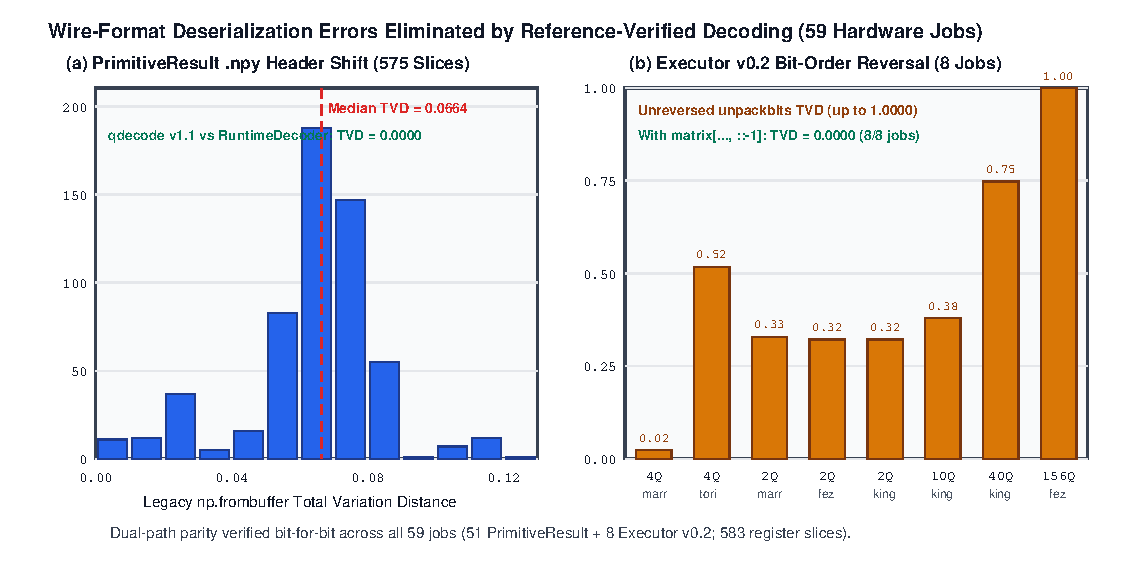
\includegraphics[width=\textwidth]{fig1_wire_deserialization_tvd_and_bit_order.pdf}
\caption{Quantitative impact of wire-format deserialization defects across all \QdTotalJobs{} archival hardware jobs (\QdTotalSlices{} register slices), contrasted against \texttt{qdecode} version~\texttt{\QdDecoderVersion} dual-path Qiskit parity ($\mathrm{TVD}=\QdRefParityTvd$). (a)~Across \QdPrimSlices{} \texttt{SamplerV2} \texttt{PrimitiveResult} slices, bypassing \texttt{np.load} with \texttt{np.frombuffer} injects the \QdNpyHeaderBytes{}-byte \texttt{.npy} header as fake shots and corrupts \QdUnalignedSlices{} row-misaligned slices, producing median $\mathrm{TVD}=\QdLegacyTvdMedian$ (maximum \QdLegacyTvdMax{}). (b)~Across all \QdExecJobs{} \texttt{Executor} \texttt{v0.2} Heron jobs (\QdExecShotsEach{} shots per job), omitting the trailing-axis reversal \texttt{matrix[..., ::-1]} after little-endian bit unpacking reverses $c_0 \leftrightarrow c_{n-1}$ and induces $\mathrm{TVD}$ from \QdExecRevTvdMin{} up to \QdExecRevTvdMax{} at \QdFezWideBits{} qubits.}\label{fig:wire_tvd}
\end{figure*}

\begin{table*}[t]
\centering
\caption{Corpus-wide deserialization and register-health audit across \QdTotalJobs{} IBM Quantum archival jobs (\QdRawDirJobs{} files in \texttt{data/raw\_jobs/} and \QdZipDistinctJobs{} distinct archives in \texttt{workloads.zip}, totaling \QdTotalCorpusShots{} PUB shots). ``Defect Med (Max) TVD'' reports the empirical total variation distance incurred by naive \texttt{np.frombuffer} header ingestion on \texttt{PrimitiveResult} payloads and unreversed little-endian bit unpacking on \texttt{Executor} \texttt{v0.2} payloads; ``Ref Parity TVD'' compares \texttt{qdecode} against Qiskit's \texttt{RuntimeDecoder} and \texttt{ExecutorResultDecoder}.}\label{tab:corpus_summary}
\begin{ruledtabular}
\begin{tabular}{llrrrrcc}
Wire schema & Format version & Jobs & Register slices & Measured & \texttt{ALL\_ZERO} & Defect Med (Max) TVD & Ref Parity TVD\\
\hline
\QdCorpusSummaryRows
\end{tabular}
\end{ruledtabular}
\end{table*}

Cloud jobs in the \QdTotalJobs{}-file corpus inhabit two structurally distinct JSON wire schemas (Table~\ref{tab:corpus_summary}):

\paragraph{\texttt{SamplerV2} \texttt{PrimitiveResult} (\QdPrimJobs{} jobs, \QdPrimSlices{} slices).} Each classical register inside a \texttt{DataBin} serializes a \texttt{BitArray} of shape $(\ldots, N, B)$ with $B = \lceil n / 8 \rceil$ packed \texttt{uint8} bytes per shot via \texttt{base64(zlib(np.save(array)))}. Critically, \texttt{np.save} prepends a self-describing binary \texttt{.npy} header beginning with magic bytes \texttt{\textbackslash x93NUMPY}, format version, and an ASCII shape/dtype dictionary padded to a 64-byte boundary (\QdNpyHeaderBytes{} bytes across all \QdPrimSlices{} archival slices). Reinterpreting the decompressed byte buffer via \texttt{np.frombuffer(..., dtype=np.uint8)} treats those \QdNpyHeaderBytes{} ASCII header bytes as leading shot outcomes while pushing \QdNpyHeaderBytes{} bytes of genuine trailing shots off the end of the array. Worse, whenever $\QdNpyHeaderBytes \bmod B \neq 0$ (occurring whenever $B \notin \{1,2,4,8,16,32,64,128\}$, such as $n=127 \Rightarrow B=16$ aligned vs intermediate 3-, 5-, 6-, 7-, or 9-byte widths, affecting \QdUnalignedSlices{} archival slices), every subsequent shot row straddles a byte boundary and garbles the entire register. Parsing exclusively through magic-validated \texttt{np.load(io.BytesIO(raw), allow\_pickle=False)} and stripping the $8B - n$ high-bit big-endian padding in byte~$0$ eliminates the \QdLegacyTvdMedian{} median TVD defect [Fig.~\ref{fig:wire_tvd}(a)].

\paragraph{IBM \texttt{Executor} \texttt{QuantumProgramResult} (\texttt{schema\_version="v0.2"}, \QdExecJobs{} jobs, \QdExecSlices{} slices).} Newer \texttt{Executor} jobs omit both \texttt{.npy} framing and (in \texttt{v0.1}/\texttt{v0.2}) \texttt{zlib} wrappers, encoding each boolean register under \texttt{data[i].results.<reg>} as
\begin{equation}
\bigl\{\texttt{"data"}: \text{base64},\; \texttt{"shape"}: [\ldots, N, n],\; \texttt{"dtype"}: \texttt{"bool"}\bigr\},
\label{eq:executor_wire}
\end{equation}
with exact byte length $\lceil N n / 8 \rceil$. Unpacking raw bytes via \texttt{np.unpackbits(np.frombuffer(raw, dtype=np.uint8), bitorder="little")[:N*n].reshape(N, n)} yields a boolean matrix $M \in \{0,1\}^{N \times n}$ whose column index $j \in \{0,\ldots,n-1\}$ corresponds to classical bit $c_j$. Because Qiskit represents bitstrings in little-endian string order $s = \text{``}c_{n-1}\ldots c_1 c_0\text{''}$ with $c_0$ rightmost—reconstructed in \texttt{qiskit-ibm-runtime} via \texttt{BitArray.from\_bool\_array(meas\_data, order="little")}—concatenating rows of $M$ directly reverses every asymmetric bitstring ($c_0 \leftrightarrow c_{n-1}$). Applying the contiguous trailing-axis reversal
\begin{equation}
M_{\mathrm{Qiskit}} = M[\ldots, ::-1]
\label{eq:axis_reverse}
\end{equation}
prior to big-endian row packing brings \texttt{qdecode} into \QdRefParityPct\% bit-exact agreement with \texttt{ExecutorResultDecoder} across all \QdExecJobs{} Heron jobs (Table~\ref{tab:executor_parity}), eliminating unreversed bit-order TVD errors of \QdExecRevTvdMin{}--\QdExecRevTvdMax{} [Fig.~\ref{fig:wire_tvd}(b)]. Six permanent regression fixtures covering symmetric, asymmetric, and multi-byte \texttt{v0.2} payloads are locked under \texttt{tests/fixtures/} to prevent future bit-order drift.

\begin{table*}[t]
\centering
\caption{Complete audit of all \QdExecJobs{} IBM \texttt{Executor} \texttt{schema\_version="v0.2"} hardware jobs (\QdExecShotsEach{} shots each across \texttt{ibm\_marrakesh}, \texttt{ibm\_torino}, \texttt{ibm\_fez}, and \texttt{ibm\_kingston}). ``Unrev.\ TVD'' compares naive unreversed \texttt{unpackbits} against Qiskit's \texttt{ExecutorResultDecoder}; ``Ref.\ TVD'' confirms exact parity after Eq.~\eqref{eq:axis_reverse}.}\label{tab:executor_parity}
\begin{ruledtabular}
\begin{tabular}{llrrrrrrrrc}
Job ID & Backend & Bits $n$ & Shots $N$ & Unique $K$ & Unrev.\ TVD & Ref.\ TVD & $H_{\mathrm{emp}}$ (bits) & $H_{\max}$ (bits) & $H_{\mathrm{emp}}/H_{\max}$ & Flag\\
\hline
\QdExecutorParityRows
\end{tabular}
\end{ruledtabular}
\end{table*}

\section{Finite-Shot Entropy Bounds and Fail-Closed Provenance}\label{sec:entropy}

\begin{figure*}[t]
\centering
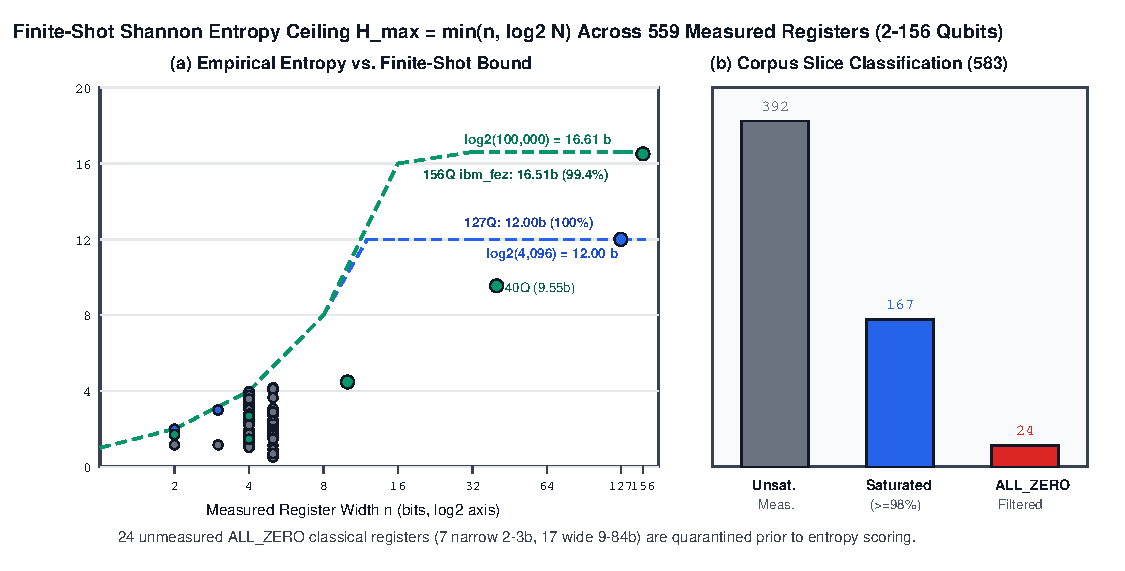
\includegraphics[width=\textwidth]{fig2_heron_59job_finite_shot_entropy_ceiling.pdf}
\caption{Finite-shot Shannon entropy scaling and register quarantine across the \QdTotalJobs{}-job corpus. (a)~Plug-in Shannon entropy $H_{\mathrm{emp}}$ versus register width $n \in [\QdMinBits, \QdMaxBits]$ across all \QdValidSlices{} valid measured registers, bounded above by $H_{\max}(n,N) = \min(n, \log_2 N)$ shown for $N=\QdArchWideShots$ ($\log_2 N = \QdArchWideCeil$\,bits, dashed blue) and $N=\QdFezWideShots$ ($\log_2 N = \QdFezWideCeil$\,bits, dashed green). Wide scrambled or noisy circuits saturate $\log_2 N$ (\QdArchWideBits{}-bit jobs \texttt{\QdArchWideJobA} and \texttt{\QdArchWideJobB} at \QdArchWideRatioPct\%; \QdFezWideBits{}-bit \texttt{ibm\_fez} job \texttt{\QdFezWideJobId} at \QdFezWideRatioPct\%) rather than $n$. (b)~Classification of all \QdTotalSlices{} decoded slices into \QdUnsaturatedSlices{} unsaturated measured registers, \QdSaturatedSlices{} finite-shot-saturated registers ($\ge \QdSatThresholdPct\%$), and \QdAllZeroSlices{} quarantined \texttt{ALL\_ZERO} unmeasured classical registers.}\label{fig:entropy_ceiling}
\end{figure*}

\begin{table*}[t]
\centering
\caption{Representative multi-scale Shannon entropy benchmarks from \QdMinBits{} to \QdMaxBits{} qubits (\texttt{prim\_res}: \texttt{SamplerV2} \texttt{PrimitiveResult}; \texttt{exec\_v02}: \texttt{Executor} \texttt{v0.2}). The rightmost column illustrates the physically meaningless shortfall $n - H_{\mathrm{emp}}$ obtained when comparing finite-shot plug-in entropy to register width $n$ instead of $H_{\max}(n,N) = \min(n, \log_2 N)$.}\label{tab:scale_benchmarks}
\begin{ruledtabular}
\begin{tabular}{lllrrrrrc}
Job ID & Backend & Schema & Bits $n$ & Shots $N$ & $H_{\mathrm{emp}} \pm \mathrm{SE}$ (bits) & $H_{\max}$ (bits) & $H_{\mathrm{emp}}/H_{\max}$ & Naive $n - H_{\mathrm{emp}}$\\
\hline
\QdScaleBenchmarkRows
\end{tabular}
\end{ruledtabular}
\end{table*}

Let $\{c_x\}_{x \in \{0,1\}^n}$ denote integer bitstring counts over $\sum_x c_x = N$ shots with empirical frequencies $\hat{p}_x = c_x / N$ supported on $K = \lvert\{x : c_x > 0\}\rvert \le \min(2^n, N)$ observed outcomes. By strict concavity of $-p \log_2 p$, the plug-in Shannon entropy~\cite{shannon1948,paninski2003} satisfies
\begin{equation}
H_{\mathrm{emp}}(\hat{p}) = -\sum_{x : c_x > 0} \hat{p}_x \log_2 \hat{p}_x \le \log_2 K \le \min\!\bigl(n,\, \log_2 N\bigr) \equiv H_{\max}(n, N),
\label{eq:entropy_ceiling}
\end{equation}
with first-order Miller--Madow bias correction~\cite{miller1955} $H_{\mathrm{MM}} = \min\!\bigl(n,\, H_{\mathrm{emp}} + \frac{K-1}{2N\ln 2}\bigr)$ and multinomial delta-method standard error
\begin{equation}
\mathrm{SE}(H_{\mathrm{emp}}) = \sqrt{\frac{1}{N}\!\left(\sum_{x : c_x > 0} \hat{p}_x (\log_2 \hat{p}_x)^2 - H_{\mathrm{emp}}^2\right)}.
\label{eq:delta_se}
\end{equation}

Equation~\eqref{eq:entropy_ceiling} exposes why comparing $H_{\mathrm{emp}}$ directly against $n$ fails catastrophically whenever $N < 2^n$ (Table~\ref{tab:scale_benchmarks} and Fig.~\ref{fig:entropy_ceiling}):
\begin{enumerate}
\item \emph{Exact collisionless saturation at $n=\QdArchWideBits$, $N=\QdArchWideShots$.} In archival jobs \texttt{\QdArchWideJobA} and \texttt{\QdArchWideJobB}, every single shot landed on a distinct \QdArchWideBits{}-bit string ($K = \QdArchWideUnique$), giving $H_{\mathrm{emp}} = \QdArchWideH$\,bits with zero plug-in variance—\QdArchWideRatioPct\% of $H_{\max}(\QdArchWideBits, \QdArchWideShots) = \QdArchWideCeil$\,bits, whereas $n - H_{\mathrm{emp}}$ would falsely report a \QdArchNaiveDeficit-bit deficit.
\item \emph{Utility-scale \QdFezWideBits{}-qubit saturation on \texttt{ibm\_fez}.} In \texttt{Executor} \texttt{v0.2} job \texttt{\QdFezWideJobId} ($n=\QdFezWideBits$, $N=\QdFezWideShots$), hardware measurements produced $K = \QdFezWideUnique$ unique bitstrings with $H_{\mathrm{emp}} = \QdFezWideHExact$\,bits ($\mathrm{SE} = \QdFezWideSE$\,bits; $H_{\mathrm{MM}} = \QdFezWideMM$\,bits) against $H_{\max}(\QdFezWideBits, \QdFezWideShots) = \QdFezWideCeilExact$\,bits—a ceiling ratio of \QdFezWideRatioPct\%, properly classified by \texttt{qscore} as \texttt{SATURATED\_ENTROPY} ($\ge \QdSatThreshold$) rather than a \QdFezNaiveDeficit-bit deficit.
\item \emph{Structured intermediate-width discrimination.} Genuine intermediate-entropy distributions remain cleanly separated below $H_{\max}$: \QdKingFortyBits{}-qubit \texttt{ibm\_kingston} job \texttt{\QdKingFortyJobId} (\QdExecShotsEach{} shots, $K=\QdKingFortyUnique$) scores $H_{\mathrm{emp}} = \QdKingFortyH$\,bits (\QdKingFortyRatioPct\% of $\QdFezWideCeil$\,bits), and \QdKingTenBits{}-qubit job \texttt{\QdKingTenJobId} ($2^{10} \ll \QdExecShotsEach$, $K=\QdKingTenUnique$) scores $H_{\mathrm{emp}} = \QdKingTenH/\QdKingTenCeil$\,bits (\QdKingTenRatioPct\%).
\end{enumerate}

Equally important, multi-register circuits frequently allocate auxiliary classical registers that are never targeted by measurement instructions and therefore return \texttt{"0"$^n$} on every shot. Across the \QdTotalSlices{} slices, \texttt{qdecode} flags and filters \QdAllZeroSlices{} \texttt{ALL\_ZERO} registers (\QdAllZeroNarrow{} narrow 2--3-bit registers and \QdAllZeroWide{} wide \QdAllZeroWideMinBits{}--\QdAllZeroWideMaxBits{}-bit registers at \QdAllZeroShots{} shots each) before statistical scoring [Fig.~\ref{fig:entropy_ceiling}(b)]. Combined with strict directory exclusions (\texttt{SKIP\_DIRS} blocking virtual-environment and \texttt{fake\_provider} paths), removal of all synthetic histogram fallbacks (failing closed with \texttt{RuntimeError} if zero valid registers load), write-protection of historical outlier CSVs, and empirical ceiling-ratio outlier detection ($\lvert z \rvert > \QdOutlierZThresh$), the pipeline guarantees that every reported metric traces cryptographically to measured QPU bitstrings.

\section{Conclusion and Data Availability}\label{sec:data}

Reliable physical inference from cloud quantum hardware archives requires treating wire deserialization and finite-shot normalization as formally verified components of the experimental apparatus. Across \QdTotalJobs{} archival IBM Quantum jobs (\QdTotalCorpusShots{} shots, \QdValidSlices{} valid measured registers, and \QdAllZeroSlices{} quarantined \texttt{ALL\_ZERO} registers), \texttt{qdecode} version~\texttt{\QdDecoderVersion} and \texttt{qscore} eliminate \texttt{.npy}-header buffer shifts, \texttt{Executor} \texttt{v0.2} little-endian bit reversals, unmeasured-register contamination, and $n \gg \log_2 N$ ceiling misclassifications with \QdRefParityTvd{} Qiskit reference discrepancy. Note that computational-basis Shannon entropy measures classical outcome dispersion only and never certifies multipartite entanglement without multi-basis Pauli witnesses (enforced separately by \texttt{qscore.ghz\_fidelity}).

Accompanying this manuscript in \texttt{papers/qdecode\_heron\_provenance\_and\_finite\_shot\_entropy/} are \texttt{generate\_qdecode\_paper\_assets.py}, \texttt{generated.tex}, the vector figures, \texttt{HARDWARE\_PROVENANCE\_MANIFEST.json} (SHA-256 prefix \texttt{\QdManifestShaPrefix\ldots}), \texttt{SHA256SUMS.txt}, and \texttt{reproducibility\_capsule.json} (RFC~8785~\cite{rfc8785} canonical SHA-256 prefix \texttt{\QdCapsuleShaPrefix\ldots}), backed by \QdPermanentFixtures{} permanent fixtures in \texttt{tests/fixtures/}.

\begin{acknowledgments}
We acknowledge the use of IBM Quantum services for the archival hardware executions analyzed in this study; the views expressed are those of the author and do not reflect the official policy or position of IBM or the IBM Quantum team.
\end{acknowledgments}

\begin{thebibliography}{9}

\bibitem{bravyi2024}
S.~Bravyi, A.~W.~Cross, J.~M.~Gambetta, D.~Maslov, P.~Rall, and T.~J.~Yoder, High-threshold and low-overhead fault-tolerant quantum memory, Nature \textbf{627}, 778 (2024).

\bibitem{nation2023}
P.~D.~Nation and M.~Treinish, Suppressing quantum circuit errors due to system variability, PRX Quantum \textbf{4}, 010327 (2023).

\bibitem{shannon1948}
C.~E.~Shannon, A mathematical theory of communication, Bell Syst.\ Tech.\ J.\ \textbf{27}, 379 (1948).

\bibitem{miller1955}
G.~A.~Miller, Note on the bias of information estimates, in \emph{Information Theory in Psychology: Problems and Methods} (Free Press, Glencoe, IL, 1955), Vol.~II-B, pp.~95--100.

\bibitem{paninski2003}
L.~Paninski, Estimation of entropy and mutual information, Neural Comput.\ \textbf{15}, 1191 (2003).

\bibitem{qiskit2026}
Qiskit Contributors, \emph{Qiskit and \texttt{qiskit-ibm-runtime}: \texttt{BitArray}, \texttt{RuntimeDecoder}, and \texttt{ExecutorResultDecoder}} (2024--2026), \texttt{https://github.com/Qiskit/qiskit-ibm-runtime}.

\bibitem{rfc8785}
A.~Rundgren, B.~Jordan, and S.~DTU, \emph{JSON Canonicalization Scheme (JCS)}, Internet Engineering Task Force RFC~8785 (2020).

\end{thebibliography}

\end{document}
